% !TeX root = ../main.tex
% -*- coding: utf-8 -*-


\chapter{基于集成学习的函数抽取重构推荐方法} 
纠错性软件维护是保证软件正确性的重要手段,然而在纠错性维护后,虽然软件系统的正确性得以保障,但对软件
系统的修改可能会导致软件系统设计的偏离,使得软件质量降低。为了提高软件质量,通常需要后续进行完善性软
件维护。为了改进软件系统的设计,经常需要在不改变代码功能的前提下改变代码的结构,这种过程通常被称为软
件重构。软件重构作为一种重要的完善性软件维护手段,可以改善软件系统的设计、提高软件的易读性和可维护性
~\cite{fowler,mens:TSE04}。

本章针对最常见的软件重构操作--函数抽取重构操作进行研究。本章首先阐述了函数抽取对完善软件系统设
计、提高软件质量的重要作用,然后介绍了本章的研究动机以及相关工作。针对研究动机中的问题描述,本章提出
了基于数据驱动的函数抽取重构推荐模型,模型中融合了内聚度、耦合度和复杂度的软件质量概念,并考虑了多种
程序元素。利用梯度上升决策树和逻辑斯特回归的融合模型,推荐函数抽取重构机会,从而帮助软件维护人员提高
维护效率。在实验部分,首先描述了实验设计,包括实验对象和评估方法。在对实验结果进行展示和分析后,讨论
了不同模型、数据集和特征对实验结果的影响,最后对本章进行小结。

\section{研究动机与相关工作}
\subsection{研究动机}
软件重构机会推荐作为一种自动化软件维护的手段,一直是研究者们较为关注的课题。软件重构机会推荐指的是推
荐软件系统中能够改善软件系统设计、提高软件质量但尚未被实施的重构机会
~\cite{fokaefs:icse11,higo:JSME,Liu:IEEE-TSE:12,Tourwe:CSMR03,Tsantalis:2011}。软件重构机会推荐可以
提高软件理解和维护的效率。Murphy-Hill等人~\cite{Murphy-Hill:ICSE09}对99个使用Eclipse集成开发工具的
Java开发人员进行了一个调研,发现函数抽取重构(Extract Method,简称EM)是最常用的软件重构类型之
一。函数抽取重构是在不改变函数功能的前提下重新组织函数,把其中部分代码片段抽取出来并组成新的函数代替原
来的代码片段被调用。函数抽取重构的原因较为复杂,包括代码重用、长函数分解、重命名内部函数等11种主要原
因~\cite{silva2016we}。虽然函数抽取重构的原因较为复杂,但通常被抽取的代码段执行一个具体的、明确的功
能。正因为此,函数抽取重构通常可以改善软件系统的设计,提高易读性和可维护性。

虽然函数抽取重构被认为是最常被使用的软件重构类型之一~\cite{Murphy-Hill:ICSE09},但根据Kim等人的调研
报告,58.3\%的被调研者手动进行所有的函数抽取重构操作~\cite{Kim:FSE12}。同样,根据JDeodorant(著名的
重构机会推荐工具)的使用统计,函数抽取重构占所有被执行的重构操作的25\%,然而只有4.4\%的函数抽取重构
时通过Eclipse集成开发环境执行~\cite{Negara:ECOOP13,Murphy-Hill:ICSE09}。研究表明,开发和设计用于自动
推荐函数抽取重构机会的推荐系统可以在集成开发环境中发挥重要的作用~\cite{Tsantalis:2011}。

为了帮助软件维护人员提高软件重构的效率,研究者们开发了针对函数抽取重构的推荐工具。由于完善性软件维
护,尤其是软件重构的主要目的是改善软件系统的设计和提高软件质量,因此大部分面向函数抽取重构机会的推荐
技术采用特定的软件质量度量作为评价重构机会的方法。目前主流的函数抽取重构机会推荐工具有:Fokaefs等人
设计的JDeodorant~\cite{fokaefs:icse11},该工具基于程序切片技术选择可以被提取到一个新函数的相关代码;
Silva等人开发的JExtract~\cite{silva:CoRR15},根据最大化内聚度和最小化耦合度的软件设计原则,设计了一
个排序函数为候选函数抽取重构机会打分,抽取相对独立的、与剩余代码依赖性较小的代码片段来组成新函数
~\cite{silva:ICPC14};类似的,Charalampidou等人提出了SEMI~\cite{charalampidou2016identifying},提取
在距离在一定范围内的相关代码片段,并根据是否存在共同变量来判断代码语句的相关性,最后针对所有的候选函
数抽取重构机会,根据软件质量度量$LCOM_2$进行排序推荐。

目前主流的函数抽取重构机会推荐方法,通过软件质量度量来评估候选重构机会的优劣,没有考虑其它与函数抽取
重构相关的因素。然而,与纠错性软件维护不同,由于软件设计的优劣和软件质量的好坏很难通过具体的公式进
行量化,因此完善性软件维护通常没有统一的、明确的标准来量化维护的效果。而以提高软件质量为目标的函数抽
取重构推荐技术,大多通过特定的软件质量度量或自定义函数对重构机会进行推荐,没有考虑到函数抽取重构原因
的多样性和复杂性,因此推荐的效果往往不甚理想。例如,软件质量度量LCOM(Lack of Cohesive Metric),只
考虑了具有共同变量的语句的个数作为内聚力的象征,而其它与函数抽取和程序功能相关的因素并没有被考虑进
去。

\begin{figure}
\centering
\subfigure[函数抽取重构前函数]{\label{fig:before}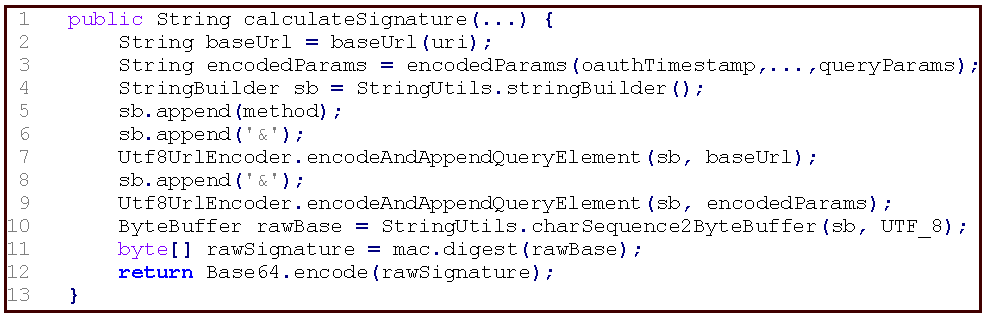
\includegraphics[width=\linewidth]{before.pdf}}
\vskip\baselineskip
\subfigure[函数抽取重构后函数]{\label{fig:after}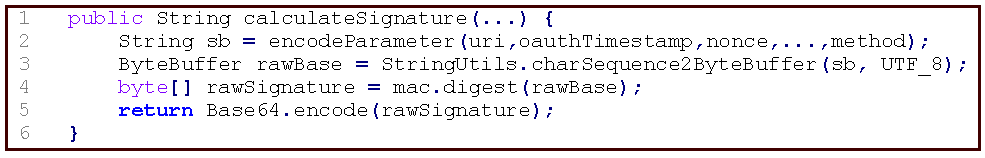
\includegraphics[width=\linewidth]{after.pdf}}
\vskip\baselineskip
\subfigure[新函数]{\label{fig:new}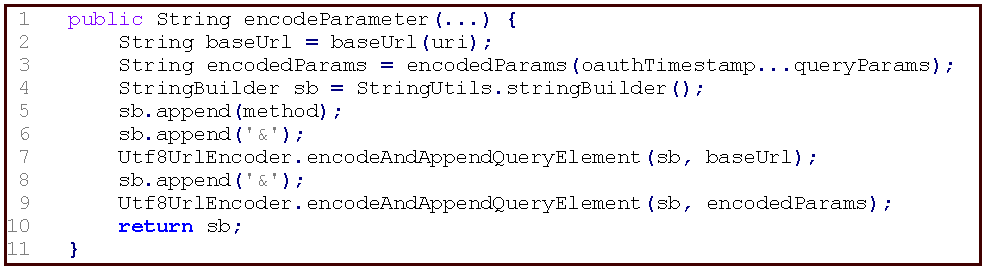
\includegraphics[width=\linewidth]{new_cropped.pdf}}
\caption{函数抽取重构示例}
\label{refactor-example}
\end{figure}

图~\ref{refactor-example}为来自AsyncHttpClient库\footnote{AsyncHttpClient为处理Java应用HTTP请求的代
码库:\url{https://github.com/AsyncHttpClient/async-http-client}}的一个简单的重构示例。图
~\ref{fig:before}为重构前的函数$calculateSignature()$,该函数的功能是计算HTTP签名。函数中第
2\textasciitilde9行实现了对参数进行编码的功能,并在接下来的版本中作为一个新的函数$encodeParameter()$
(图~\ref{fig:new})被提取出来。图~\ref{fig:after}为函数抽取重构后的函数,可以看到在第2行通过调用新
函数,保持函数的语义和功能不发生改变。

\begin{table}[!t]
\zihaowu
  \renewcommand{\arraystretch}{1.3}
  \caption{示例函数的函数抽取重构机会}
  \label{example_metrics}
  \centering
  \begin{tabular}{ccccc|ccccc}
  \toprule No.&Can&LCOM$_1$&LCOM$_2$&CPL &No.&Can&LCOM$_1$&LCOM$_2$&CPL\\ \midrule 1 &2-7 &8 &0 &6
   &9 &3-10 &6 &0 &6\\
   2 &2-8 &10 &0 &6 &10 &3-11 &13 &0 &6\\
   3 &\textbf{2-9} &11 &0 &6 &11 &3-12 &21 &0 &6\\
   4 &2-10 &13 &0 &6 &12 &4-9 &0 &0 &3\\
   5 &2-11 &28 &3 &6 &13 &4-10 &0 &0 &3\\
   6 &2-12 &36 &10 &6 &14 &5-7 &0 &0 &3\\
   7 &3-8 &4 &0 &6 &15 &5-8 &0 &0 &3\\
   8 &3-9 &5 &0 &6 &16 &5-9 &0 &0 &4\\
   \bottomrule
  \end{tabular}
\end{table}

为了模拟基于软件质量度量的函数抽取重构过程,表~\ref{example_metrics}中列出了函数$calculateSignature$
(如图~\ref{fig:before}所示)的16个候选函数抽取重构机会以及对应的软件质量度量。其中,Can为候选重构机
会,表~\ref{example_metrics}中使用起止代码行号来表示可被抽取的函数代码片段。表中列出了三种软件质量度
量方法,分别是函数内聚力缺乏度LCOM$_1$、LCOM$_2$和耦合度~\cite{yang2009identifying}。值得注意的是,
函数抽取重构中通常使用的LCOM$_1$和LCOM$_2$为描述函数体内部凝聚力的软件质量度量
~\cite{charalampidou2015size}。给定代码段$B$,$P$表示代码段中不共享任何变量的语句对的个数,$Q$为代码
段中存在共同变量的语句对的个数,则有$LCOM_1=P$。LCOM$_2$计算方式如下:
\begin{equation}\label{eq:lcom2}
      LCOM_2 = 
       \begin{cases}
             P-Q, & \textit{if}~P-Q\geq 0\\ 
  0, & elsewise,  
       \end{cases}
\end{equation}
不难看出,从函数体中抽取一个代码段,该代码段的LCOM$_1$和LCOM$_2$的值越低,表示其中不共享变量的语句对
越少,共享变量的语句对越多,此时代码段的内聚力越强。表~\ref{example_metrics}中的耦合度为抽取该代码段时
所需要的参数的个数~\cite{yang2009identifying},因此耦合度越低,表示此时需要的参数越少,代码段与重构后
的原函数相关性较低,更符合软件设计原则。为由于示例代码的结构较为简单,因此表~\ref{example_metrics}中
未列出关于复杂度的软件质量度量。根据图~\ref{refactor-example}可知,在列出的16个函数抽取重构机会中只
有第3个重构机会(第2\textasciitilde9行)代表了最终抽取的代码片段。从表~\ref{example_metrics}中可以看
出,第12\textasciitilde16个代码段具有更低的函数内聚力缺乏度和耦合度,因此根据软件质量度量更适合被抽
取出来组成新函数;相反,相比较其它候选重构机会,第3个代码段在三个度量标准上均未有明显的优势,因此很
难通过软件质量度量来解释该代码段在后续版本中被抽取出来的原因。

因此,利用特定的软件质量度量来推荐函数抽取重构机会存在一定的局限性:(1)虽然软件质量度量是为了评价
软件质量而设计的,然而现有的度量标准往往只考虑某一种特定的程序元素,例如LCOM只考虑了使用共同变量的语
句的个数,而其它与软件质量相关的程序元素,如函数调用、类型和包等并没有被考虑进去。(2)函数抽取的目
的并不仅仅是为了提高软件质量度量或是减少代码坏味,还包括缺陷修复、方便新功能的添加或者提高程序易读性
等很难被量化的目的。因此通过某个软件质量度量或预定义的公式来进行函数抽取重构推荐,容易导致推荐的不准
确性。本章提出通过学习开源软件仓库中的重构实例,挖掘函数抽取重构的原因,构建关于函数抽取重构的概率模
型来推荐函数抽取重构机会。

本章提出基于机器学习的函数抽取重构机会推荐模型,通过提取一组结构特征和一组功能特征来对候选函数抽取重
构机会进行表示。具体来说,在特征提取算法中,提取了一组与函数和候选代码片段的复杂度相关的结构特征,以
及一组与内聚度和耦合度相关的功能特征。与传统的软件质量度量不同,该模型将软件质量相关的特征用一系列程
序元素来表示,包括与代码功能相关的变量使用、函数调用和包等。通过融合多种软件质量概念和程序元素,将函
数抽取重构机会表示为可供学习的特征序列。通过从开源软件仓库中挖掘真实存在的函数抽取重构实例,模型可以
从中学习到关于函数抽取重构的概率模型。给定一个新的函数体,该模型生成的候选函数抽取重构机会,并为每个
合法的重构机会分配一个概率,表示该重构机会为使用者所采纳的可能性,并按照概率由高至低进行推荐。

\subsection{相关工作}
函数抽取重构推荐主要分为两个步骤:给定待重构的函数体,首先识别可以被抽取的代码段作为候选重构机会,然
后根据某种特定的方式将候选重构机会进行排序,并按序推荐给软件维护人员。因此,根据函数抽取重构的过程,
可以将关于函数抽取重构推荐的研究分为两个部分,分别是函数抽取重构机会识别和排序。本节从上述两个角度来总结和分析当前主流的函数抽取重构机会推荐方法。

\subsubsection{函数抽取重构机会识别}

函数抽取重构机会识别指的是识别函数体中可以抽取的代码从而组成一个新的函数的代码,其本质是对函数体进行
拆分。目前关于识别函数抽取重构机会的研究主要分为基于程序语法和语义两种。

基于程序语法的函数抽取重构机会识别,主要通过程序切片的方式保证程序语法的正确性。Maruyama等人
~\cite{maruyama2001automated}首次提出使用程序切片来识别函数抽取重构机会,提出了个基于基本代码块的切
片方法对程序的控制流图进行切片。虽然该方法利用基本块来限制程序切片的范围,但由于其无法从语法上保证抽
取代码段前后程序的行为保持一致,因此其实用性受到了限制。为了保证函数抽取重构不会使程序行为发生改变,
Tsantalis和Chatzigeorgious~\cite{tsantalis2011identification}针对给定变量和对象,通过计算程序切片得
到所有可能改变变量的值或对象的状态的可执行切片。通过对程序切片的完全计算,该方法能够对给定的切片要求
(如某个特定的变量),在提取出所有与指定要求相关的代码片段的同时不改变原来的程序行为。

除了程序切片外,Yang等人~\cite{yang2009identifying}提出了针对规模较大的函数(``长函数''代码坏味)的
函数拆分方法,该方法根据函数的层次结构(如空行、分支和循环等)将长函数拆分成多个代码片段作为函数抽取
重构机会。Meananeatra~\cite{meananeatra2011using}等人定义了一组关于程序控制流和数据流的布尔表达式来
筛选被抽取的代码段,从而保证程序行为不变。例如,通过限制变量的定义和使用关系,确保变量在使用前已经被
定义,该方法可以过滤掉只包含某个变量的使用而不包含该变量定义的代码片段。Silva等人
~\cite{silva:ICPC14,silva:CoRR15}提出了基于代码块的函数抽取重构机会生成算法,将函数体表示为具有层次
结构的代码块的组合,每个代码块由顺序执行的子代码块组成。针对每个代码块,其中连续的子代码块组成一个候
选函数抽取重构机会。通过这样的方式,该算法能够生成所有能够顺序执行的代码片段,最终通过规则筛选出所有
合法的函数抽取重构机会。

基于程序语法的函数抽取重构机会识别,通常只能保证函数抽取重构后程序的语义和功能不发生改变,但仍然依赖
软件维护人员判断如何选取函数抽取重构机会(或指定切片条件)。根据``一个功能原则
''~\cite{martin2003agile}(Single Responsibility Principle,SRP),软件系统内的每个函数应该完成一个明确
的、特别的功能。基于这个原则,Charalampidou等人~\cite{charalampidou2016identifying}认为应该识别可能
完成某个特定功能的代码片段进行函数抽取重构。具体来说,他们认为在距离相近的有共同变量或函数调用的代码
语句在完成同一个功能,因此将这些语句视为一簇;通过合并重叠的小簇形成大簇,然后将每个大簇作为一个候选
重构机会。通过这种方法,他们认为能够识别所有可能在执行同一个程序功能的代码片段。然而,该方法在限制代
码之间距离的同时也限制了被抽取的代码片段的规模。例如,在代码片段中位置比较靠前的变量声明语句,由于距
离变量的使用存在一定距离,因此经常容易被忽略。除此以外,该方法在考虑代码功能的时候只考虑了变量和函数
调用,而没有考虑其它和代码功能相关的程序元素,如类型、包等。

\subsubsection{函数抽取重构机会评价}

函数抽取重构是从给定函数体中抽取代码片段组成新函数并调用的过程。然而,能够抽取并保持程序行为不变的代
码片段通常有很多,尤其当函数规模变大时,其函数抽取重构机会的数量往往呈指数级上升。为了提高软件维护的
效率,部分研究对函数抽取重构机会进行排序,然后按序将候选重构机会推荐给使用者。

目前大部分关于函数抽取重构机会推荐的研究是根据函数级软件质量度量来对候选重构机会进行排序。软件质量度
量为从质量角度对软件系统的度量,其中与函数抽取重构相关的主要有复杂度、内聚度和耦合度等。根据SRP原
则,理想的函数抽取重构可以降低原函数的复杂度,使原函数和新函数内聚度尽可能高、耦合度尽可能低。

具体来说,基于复杂度的概念,部分研究使用函数复杂度(Method Complexity,MCX)来对函数抽取重构机会进行
排序~\cite{meananeatra2011using, yang2009identifying},倾向于推荐可以使函数复杂度尽可能小的重构机
会。基于内聚度的概念,部分研究使用函数内聚缺乏度(Lack of Cohesion of Method,LCOM)来评估函数抽取重
构对软件质量的改进程度,优先推荐让原函数和新函数的函数内聚缺乏度尽可能低的函数抽取重构机会
~\cite{meananeatra2011using, charalampidou2016identifying}。基于耦合度的概念,部分研究者提出优先推荐
尽可能独立的代码片段,使得重构之后原函数和新函数相关性尽可能小
~\cite{yang2009identifying,silva:ICPC14,silva:CoRR15},例如可以通过计算函数抽取时新函数所需要的参数
的数量来评估新函数对原函数的依赖性~\cite{yang2009identifying}。

与基于软件质量度量的方法不同,考虑到函数抽取重构原因的多样性~\cite{silva2016we}和软件质量度量的局限
性,本章提出构建关于函数抽取重构的概率模型,挖掘开源软件仓库中学习的重构实例,从中学习如何进行函数抽
取重构;除此以外,开发了``生成-排序''的推荐系统,为给定函数体生成所有合法的函数抽取重构机会,然后使
用训练好的模型为每个重构机会分配一个概率作为分数,按照分数由高至低进行推荐。与本章工作最相近的是
Silva等人的JExtract~\cite{silva:ICPC14,silva:CoRR15},该方法与本章方法的共同点是在识别函数抽取重构机
会的阶段不对重构机会进行筛选,而是依赖于后续的排序方法为使用者推荐重构机会;最大的区别是JExtract中的
排序算法假设被抽取的代码片段应该尽可能独立,因此JExtract计算待抽取代码与剩余代码之间的结构依赖性,推
荐尽可能独立的代码片段进行函数抽取重构。然而,软件维护人员进行函数抽取的原因多种多样
~\cite{silva2016we},只考虑结构依赖性作为函数抽取的原因在某些情况下存在一定的局限性。

\section{研究方法}
软件重构是完善性软件维护的重要手段。针对最常见的软件重构类型之一--函数抽取重构,本文提出了基于梯度上
升决策树的函数抽取重构机会推荐方法,并开发了基于Eclipse的插件GEMS。本节首先介绍了方法的基本框架,然
后提出了针对函数抽取重构实例的特征提取算法,接着阐述了本文使用的梯度上升决策树和逻辑斯特回归融合模
型,最后针对预测阶段给定函数体,阐述了基于代码块的候选函数抽取重构机会生成的方法,并描述了模型预测和
排序的过程。

\subsection{基本框架}
基于梯度上升决策树的函数抽取重构机会推荐,主要包括模型训练和重构推荐两个阶段。

\subsubsection{训练阶段}

为了挖掘函数抽取重构的原因,本章提出基于数据驱动的函数抽取重构机会推荐,通过对比开源软件仓库中两个相
邻的提交版本,收集函数抽取重构实例作为样本。然后针对训练样本集中的函数抽取重构实例进行特征提取,根据
特征提取算法将其表示为一个特征向量(feature vector)。最后训练模型。在将训练样本通过特征提取算法表示
完成后,利用基于梯度上升决策树和逻辑斯特回归的融合模型进行训练。


\subsubsection{推荐阶段}

给定函数体,首先基于代码块的函数抽取重构机会生成算法,将所有在一个代码块内的连续子块作为可能的函数抽
取重构机会。然后筛选函数抽取重构机会。由于基于代码块的重构机会生成算法可能生成破坏程序语义和功能的重
构机会,因此使用基于规则的方法对函数抽取重构机会进行筛选,得到由所有合法重构机会组成的集合。最后对函
数抽取重构机会进行预测和排序推荐。针对集合中的每一个函数抽取重构机会,使用训练好的模型预测其为训练样
本中正例的概率,并根据概率由高至低进行排序,按序推荐给使用者。

值得注意的是,虽然本章方法需要一定的训练时间,但由于该训练过程是离线的,在训练完成后可以直接部署在集
成开发环境中,由使用者指定需要重构的函数,使用训练好的参数进行重构推荐,因此效率较高。

\subsection{相关定义与特征提取算法}
\subsubsection{相关定义}

\begin{Definition}
  函数抽取重构机会。给定函数$m$,$c$为函数$m$中由连续语句组成的代码片段,若代码片段$c$能够被抽取
  出来组成一个新的函数,并在原函数$M$中以同样的方式调用,使原函数$m$的功能和语义保持不变,则代码片段
  $c$为函数$m$的一个函数抽取重构机会。
\end{Definition}

\begin{Definition}
  函数-重构机会对。函数$m$和其中一个函数抽取重构机会$c$组成了一个函数-重构机会对$p$,记为$p=(m,c)$。
\end{Definition}

\begin{Definition}
  函数抽取重构实例。给定函数$m$,若其中的一个函数抽取重构机会$c$在后续的版本中被提取出来进行函数抽取
  重构,则函数$m$和$c$组成一个函数抽取重构实例$r$,记为$r=(m,c)$。
\end{Definition}

本文通过比较开源软件仓库中的相邻版本得到的真实的函数抽取重构实例集$\mathcal R$。给定训练样本集
$\mathcal D$,其中第$i$个样本记为$\mathcal D^{(i)}=(x^{(i)},y^{(i)})$,$x^{(i)}$表示样本数据,为一个
函数-重构机会对,即$x^{(i)}=p^{(i)}=(m^{(i)},c^{(i)})$;$y^{(i)}$表示样本的标签,即该函数-机会对是否
为函数抽取重构实例。因此样本标签$y^{(i)}$可以表示为:
\begin{equation}
   y^{(i)} = 
       \begin{cases}
             1, & \textit{if}~p^{(i)}\in \mathcal D\\ 
  0, & elsewise,  
       \end{cases}
\end{equation}

为了学习关于函数抽取重构的概率模型,首先对样本$D^{(i)}\in\mathcal D$的输入数据$x^{(i)}$表示成特征向
量$x^{(i)}=(x^{(i)}_1,x^{(i)}_2,...,x^{(i)}_n,)$,其中$n$为特征的个数。针对每个函数-重构机会对,通过静态
分析提取关于结构和功能的两组特征。尽管本文方法不是为了推荐满足某个特定软件质量度量的函数抽取重构机
会,但根据SRP原则,本文的特征提取算法中融合了包括复杂度、内聚度和耦合度在内的软件质量因素,并考虑了
多种程序元素。值得注意的是,虽然在特定情况下函数抽取也被用来防止代码重复,但针对以避免代码重复为目的
的函数抽取重构并不在本文的研究范围内,因为在研究中通常使用代码克隆检测技术来避免代码重复
~\cite{bellon2007comparison}。

\subsubsection{结构特征}

给定由函数$m$和重构机会$c$组成的函数-重构机会对$p$,首先根据函数抽取重构机会将函数$m$分为两部分:待抽取
的代码片段和剩余代码。对每部分代码$g$,GEMS提取其控制流图$graph(g)$,并计算其函数复杂度(MCX):
\begin{equation}
   MCX(g) = E(g) - N(g) + 2P(g)
\end{equation}
其中,$E(g)$表示控制流图$graph(g)$中边的个数,$N(g)$表示$graph(g)$中节点的个数,$P(g)$表示$graph(g)$
中连通分支的个数。通过这样的方式,计算出待抽取代码片段和剩余代码的函数复杂度。除软件度量外,GEMS还通
过简单的程序分析提取了其它与代码复杂度相关的特征。如根据控制流语句得到代码片段中各种代码结构(如分支
结构、循环结构)的数量;根据变量、类型、函数调用等,得到关于代码片段中各种程序元素的数量。本文从直观
上认为使用更多的变量、类型、循环等程序元素的代码片段通常更加复杂,因此易读性和易理解性更低。

值得注意的是,GEMS虽然提取了一组跟复杂度相关的结构特征对样本进行表示,但并没有假设其中的每个特征均与
模型预测结果相关,特征与是否进行函数抽取重构之间的关系仍需要依赖模型训练学习得到。换言之,提取的特征
只是可能与函数抽取重构相关的特征,但不能保证不存在``冗余特征''。关于特征对模型的影响和特征选择的分
析,本文会在~\ref{discuss}通过实验进一步讨论和分析。

除此以外,之前的研究通过设置阈值来限制被抽取代码的规模
~\cite{silva:ICPC14,charalampidou2016identifying}。与之前的研究不同,GEMS通过计算被抽取代码行数占总
代码行数的百分比作为特征,让模型学习函数抽取重构机会与代码规模的关系。通过这样的方式,GEMS提取被抽取
的代码片段的规模作为特征,让模型在推荐阶段能够过滤掉抽取过量或极少量代码的函数抽取重构机会。例如,通
过实验发现,大部分只抽取一行代码和几乎抽取整个函数体的重构机会被分配到较低的概率,因此很少被推荐给使
用者。

\subsubsection{功能特征}

由于函数抽取重构的过程是将原函数中的代码段抽取出来组成一个新函数,而同时根据SRP原则,每个函数应该完
成一个独立的、明确的函数功能,因此,虽然函数抽取重构的原因较为复杂和多样,但通常被抽取的代码段在功能
上应该相对独立。另一方面,调查发现,函数抽取重构的主要目的之一将原函数功能拆分成多个子功能,每个子功
能完成一个相对独立的功能,从而提高软件系统的易理解性和可维护性~\cite{silva2016we}。因此,除了结构特
征外,GEMS还提取了一组与功能相关的特征。

给定函数-重构机会对$p=(m,c)$,GEMS提取了一组功能特征来判断函数抽取重构机会$c$是否选择一个独立的、内
聚的、具有某个函数子功能的代码段。具体来说,对代码段功能特征的提取主要分为两步:
\begin{itemize}
  \item 基于耦合度的概念,提取函数抽取重构机会$c$中可能完成的、剩余代码$m-c$中所未提供的函数
  子功能$q$;
  \item 基于内聚度的概念,计算函数抽取重构机会$c$所选择的代码段对函数子功能$q$的凝聚度,即被抽取的代
  码对子功能$q$的投入程度。
\end{itemize}

具体而言,对于函数-重构机会对$p=(m,c)$中的待抽取代码段,GEMS首先提取其可能独立执行的某个函数子功能,
具体方式是寻找只出现或主要出现在待抽取代码段中的程序元素。传统的软件质量度量只考虑特定的程序元素作为
评价软件质量的方法,例如LCOM$2$中只考虑不同语句对变量的使用来推断它们的相关性。与传统的软件质量度量
不同,本文考虑了与程序功能相关的变量、函数调用、类型、包四种程序元素类型。之所以在特征提取阶段考虑多
种程序元素,是因为除了变量外,完成一个功能通常还涉及到类型、函数调用、代码库等多种程序元素
~\cite{martin2003agile},而部分程序元素可能比变量本身更能体现代码所执行的功能。对每种程序元素类型,
本文首先寻找该类别中在待抽取代码段和剩余代码段中出现频率相差最大的具体程序元素,作为可能代表待抽取代
码的独立子功能的程序元素。然后,在从待抽取代码段中提取出可能代表其独特子功能的程序元素后,接下来就是
计算该代码段对函数子功能的投入程度。与传统的软件质量度量不同,本文在对代码段对函数子功能的投入程度时
综合考虑了多种程序元素,因此对于上一步骤中提取出来的最有可能代表代码段独特子功能的每个程序元素,本文通过
计算代码段中使用到该程序元素的语句占待抽取代码段语句的比例,来计算代码段对该独特子功能的投入程度。

算法~\ref{alg:feature}描述了提取功能特征的过程。给定函数-重构机会对$p=(m,c)$,其中$m$为原函数,$c$为
函数重构机会,$b$为该重构机会中待抽取的代码片段,GEMS首先获取$m$和$b$中的语句,得到集合$S_m$和$S_b$
(第1\textasciitilde2行)。然后,对于程序元素类型集合$W$中的每种程序元素类型$w$,首先基于耦合度的概
念,提取该类型中最独特的程序元素$e^*$(第6\textasciitilde14行);然后基于内聚度的概念,计算待抽取代
码中该程序元素被使用的程度(第15\textasciitilde23行);最后将这两类特征分别放到特征向量中(第24
行)。

其中,程序元素类型$W$主要包括四种:变量、类型、函数调用和Java包。对于每一种程序元素类型$w$,首先获取
待抽取代码$b$中所有该类型的程序元素$E_w$(第7行);然后针对其中的每种程序元素$e$,分别计算该元素在函
数$m$和代码段$b$中出现的频率$freq_m$和$freq_b$(第9\textasciitilde10行),并计算频率的比例$ratio_e$
(第11行);通过选择具有最大$ratio$的程序元素,得到该类型中最主要在待抽取代码中出现的程序元素$e^*$
(第13行)。以Java包为例,如果某个Java包只在待抽取代码中被使用,则该Java包对应的$ratio$为1,此时该类
型的$cp$也为1(第14行)。通过这种方式,提取到可能代表待抽取代码段独特子功能的4种程序元素。需要声明的
是,为了容易理解,在算法~\ref{alg:feature}中为每种类型只选择了一个程序元素,而在实际模型中对每类程序
元素选择$ratio$最大的两个元素计算$cp$作为耦合度相关特征。最后对上述可能代表程序子功能的程序元素,分
别计算在待抽取代码段$b$中使用的程度(第15\textasciitilde23行),若某个程序元素出现在代码段$b$中的每
个语句中,则此时对应的$ch$为1,说明此时待抽取代码段的内聚力较高。最后对每类程序元素分别计算得到$cp$
和$ch$后,将其作为功能特征向量返回。通过这种方式,针对给定函数和待抽取代码段,该算法能够抽取出代码段
可能完成的独特的函数子功能,从而通过特征提取将内聚度和耦合度的概念融入到模型中。

\begin{algorithm}[H]
\caption{功能特征提取算法}\label{alg:feature}
\KwIn{函数$m$,待抽取代码片段$b$,程序元素类型序列$W$;}
\KwOut{功能特征向量$f$;}
获取函数$m$中的所有语句$S_m$;\\
获取代码片段$b$中的所有语句$S_b$;\\
\For {$w$ in $W$} {
  //对每种程序元素类型$w$进行计算\\
  获取待抽取代码段$b$中的所有类型为$w$的程序元素,得到序列$E_w$;\\
  \For {$e$ in $E_w$} {
    统计程序元素$e$在函数$m$中出现的频率$freq_m$;\\
    统计程序元素$e$在代码段$b$中出现的频率$freq_b$;\\
    计算$ratio_e = freq_b/freq_m$;\\
  }
  选择$E_w$中$ratio$最大的程序元素$e^*$;\\
  令$cp_w = ratio_{e^*}$;\\
  计算代码段$b$的代码行数$loc = getLOC(b)$;\\
  初始化$count = 0$;\\
  \For {$s$ in $S_b$} {
    //对代码段$b$中的每个语句\\
    \If {$e^*$ in $s$} {
      更新$count = count + 1$;\\
    }
  }
  计算$ch_w = count/loc$;\\
  将$cp_w$和$ch_w$设置为程序元素$w$的两个功能特征。\\
}
\end{algorithm}
\subsection{梯度上升决策树}
给定训练数据集$\mathcal D$中的第$i$个样本${\mathcal D}^{(i)}=(x^{(i)},y^{(i)})$,通过特征提取将$x^{(i)}$
其表示为$x^{(i)}=\{x_1^{(i)},x_2^{(i)},...,x_n^{(i)}\}$;$y^{(i)}$为第$i$个样本的类别,$y^{(i)}=1$表
示第$i$个样本为正样本,$y^{(i)}=0$表示第$i$个样本为负样本。在将训练数据集表示为特征向量和标签后,构
建基于梯度上升决策树的二分类模型,通过使用$Logloss$作为损失函数,拟合样本为正样本的概率;在推荐阶
段,使用训练完成的模型为给定函数抽取重构机会预测其为正样本的概率,并按照概率由高至低推荐函数抽取重构
机会。

首先简单阐述基于梯度上升决策树的原理。梯度上升决策树为基于多个弱学习器的融合模型,由于梯度上升决策
树的目标是为给定样本预测一个连续值,因此其使用的弱学习器为回归树。梯度上升决策树的优点在于:(1)通
过融合多个弱学习器,得到对性能的显著提升;(2)在训练阶段,可以保持现有模型不变,通过增加新的弱学习
器(决策树),提高模型的表现,使用较为灵活;(3)能够发现有效的特征组合。具体来说,本文使用CART回归
树作为弱学习器,在节点分裂的时候使用最小均方差(Mean Squared Error,MSE)作为分裂准则,选择使每个分
支的均方差之和最小的条件作为节点分裂的条件。

本文使用的基于梯度上升决策树的二分类模型,因此选用$Logloss$作为损失函数:
\begin{eqnarray}
  Loss(y^{(i)},F_k(x^{(i)})) = -(y^{(i)}logp^{(i)} + (1-y^{(i)})log(1-p^{(i)})),
\end{eqnarray}\label{logloss}
其中$F_k(x^{(i)})$表示$x^{(i)}$在以前$k$棵树作为模型时的预测结果,根据罗基斯特方程,$p^{(i)}$为
$x^{(i)}$为正样本的概率:
\begin{eqnarray}
  p^{(i)} = \frac{1}{1 + e^{-F_k(x^{(i)})}}.
\end{eqnarray}
梯度上升决策树通过每次新增一个树$F_k$来拟合损失函数的负梯度在当前模型$F_{k-1}$的取值。

\subsection{函数抽取重构机会推荐}
在推荐阶段,对于给定函数,首先生成所有可能的函数抽取重构机会,然后通过基于规则的方法过滤掉可能改变程
序行为的代码片段,得到所有合法的函数抽取重构机会后,使用训练好的梯度上升决策树模型为合法重构机会分配
概率,并按照概率由高至低推荐给用户。

\subsubsection{函数抽取重构机会生成}
本文的函数抽取对象为连续语句构成的代码片段,因此给定函数,需要在不破坏程序语法的前提下,生成所有可能
的函数抽取重构机会,通过分析函数的控制流结构,生成代码结构树,并通过对代码结构树的遍历得到所有可能的
函数抽取重构机会。

\begin{figure} 
  \centering 
  \begin{minipage}[c]{0.5\textwidth} 
    \centering 
    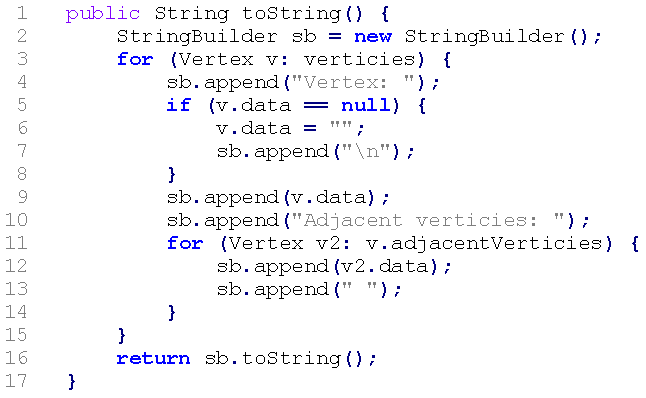
\includegraphics[width=3in]{block.pdf} 
  \end{minipage}% 
  \begin{minipage}[r]{0.5\textwidth} 
    \centering 
    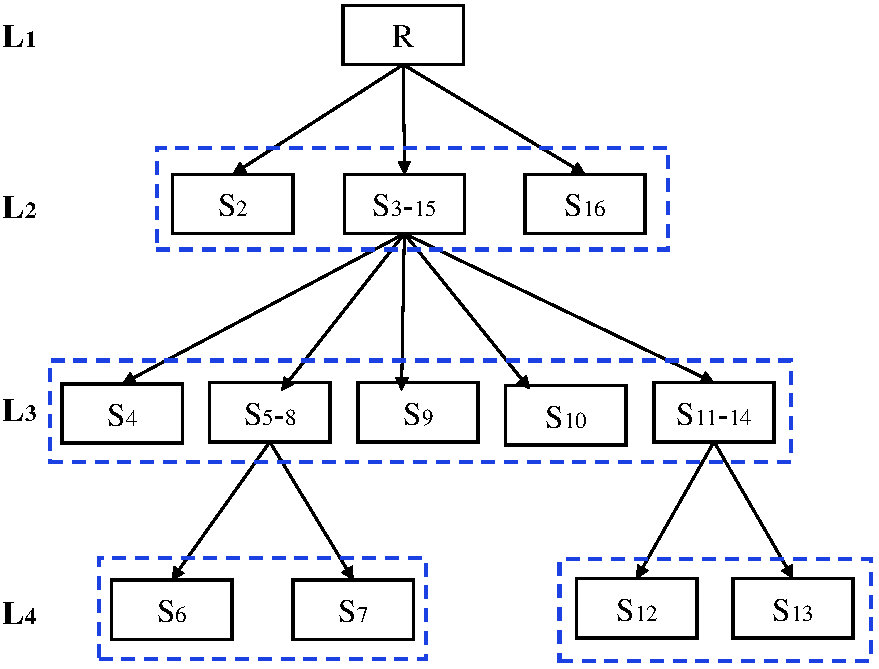
\includegraphics[width=2in]{block_structure.pdf} 
  \end{minipage} 
\caption{示例代码的结构表示}
\label{block-example}
\end{figure}

图~\ref{block-example}为示例代码及其代码结构树,其中代码结构树中的$S_j$指代的是示例代码的第$j$行代
码。可以看到,示例代码的代码结构树高度为4,其中包括根节点在内,共有4个非叶子结点,分别为$R$、
$S_{3-15}$、$S_{5-8}$和$S_{11-14}$,每个非叶子节点表示代码内部的一个控制结构,在图
~\ref{block-example}中用蓝色虚线框表示。以根节点$R$为例,$R$的3个子节点分别为$S_2$、$S_{3-15}$和
$S_{16}$,表示函数$toString()$一共包括3条语句,依次为语句$S_2$、$for$循环语句$S_{3-15}$和语句
$S_{16}$。通过对代码结构树进行遍历,针对树中的每个非叶子结点,生成由连续子节点组成的代码片段,得到所
有可能的函数抽取重构机会。

以根节点为例,根节点的子节点从左到右依次为$Child(R)=\{S_2,S_{3-15},S_{16}\}$。由于根节点共有3个子节
点,因此可以依次生成长度为1的连续语句:$\{\{S_2\},\{S_{3-15}\},\{S_{16}\}\}$、长度为2的连续语句
$\{\{S_2,S_{3-15}\},\{S_{3-15},S_{16}\}\}$和长度为3的连续语句:$\{\{S_2,S_{3-15},S_{16}\}\}$。最后可
以得到,根据代码块$B_1$生成的代码片段有
$cf(B_1)=\{\{S_2\},\{S_{3-15}\},\{S_{16}\},\{S_2,S_{3-15}\},\{S_{3-15},S_{16}\},\{S_2,S_{3-15},S_{16}\}\}$。
通过同样的方式,遍历4个非叶子结点后一共得到27个由连续语句组成的代码片段作为潜在的函数抽取重构机会。
需要注意的是,对于非叶子结点而言,其子节点可以是普通语句或是结构语句(如分支、循环等),例如根节点
$R$的第二个子节点为一个$for$循环语句。

\subsubsection{函数抽取重构机会筛选}
由于函数抽取重构的前提是不改变程序的语义和行为,因此为了避免重构后发生编译错误,需要对基于代码块生成的所有可能的函数抽取重构机会进行筛选,过滤掉以下情况:
\begin{itemize}
  \item 根据Java编程语言的要求,每个函数不能有超过一个返回值,因此要过滤掉那些在抽取函数后需要返回不
  止一个值到原函数的函数抽取重构机会;
  \item 由于类型的声明和使用应该在一个代码块中,因此要过滤掉导致类型的声明和使用被分开的函数抽取重构
  机会,例如某个类型的声明语句被抽取而对于该类型的使用仍然留在原函数中;
  \item 如果被抽取的代码片段中含有$continue$、$break$或者$case$等语句,然而却不包含与其相配套的代码
  结构,则该函数抽取重构机会被视作非法的,应当被过滤掉。
\end{itemize}

\subsubsection{预测与排序}
在推荐阶段,给定函数$m$后,为其生成所有合法的函数抽取重构机会$P(m)$,根据特征提取算法,为每个函数
抽取重构机会$p\in P(m)$提取一个特征向量$f(p)$作为输入数据$x(p)$,使用训练好的模型参数预测该特征向量
的输出$y(p)$,$y(p)$表示函数抽取重构机会$p$为正例的概率。在对每个合法函数抽取重构机会分配一个概率
后,按照概率由高至低将函数抽取重构机会推荐给用户。需要注意的是,在实际应用中用户很难看完所有的重构机
会再进行选择,因此在使用中通常只推荐排名最高的若干个函数抽取重构机会。

\section{实验设计}
在基于梯度上升决策树的函数抽取重构机会推荐模型的基础上,开发了基于Eclipse的开源工具GEMS\footnote{http://www.comp.nus.edu.sg/~specmine/gems}。为了评估方法的有效性,通过在5个开源软件上进行
实验,对比评估了GEMS与其它3种当前流行的函数抽取重构机会推荐方法,证明了本文的有效性。除此以外,
还设计了关于模型选择和特征重要性的实验,并对实验结果进行了讨论和分析。

\subsection{对比方法与实验对象}
为了评估本章方法的有效性,与3个当前流行的函数抽取重构机会推荐工具进行对比实验,这三个工具分别是:
\begin{itemize}
  \item JExtract~\cite{silva:ICPC14,silva:CoRR15},该工具同样也是一个``生成-排序''系统,与本章方法的
区别是JExtract使用自定义的函数为每个函数抽取重构机会打分,而GEMS通过构建概率模型学习如何进行函数抽取
重构。
  \item SEMI~\cite{charalampidou2016identifying},该方法通过识别连续的相关的代码语句作为候选函数抽取
机会,并按照软件质量度量LCOM$_2$的高低进行排序并推荐。
  \item JDeodorant~\cite{tsantalis2011identification},该工具通过计算程序切片得到所有可能改变变量的
  值或对象的状态的可执行切片作为候选函数抽取重构机会进行推荐。
\end{itemize}

本章的实验对象为5个开源软件,分别是JHotDraw、Junit、MyWebMarket、SelfPlanner和WikiDev。其中
JHotDraw、Junit和MyWebMarket为文献~\cite{silva:ICPC14}中用来证明JExtract有效性的实验对象,
SelfPlanner和WikiDev与文献~\cite{tsantalis2011identification}中用来证明JDeodorant有效性的实验对象相
同,而文献~\cite{charalampidou2016identifying}使用了这5个软件系统来评估SEMI的有效性。表
~\ref{benchmark}为这5个开源软件系统的统计信息。可以看到,在这5个开源软件中的共有130个函数存在函数抽
取重构操作,而实验的目标是为这130个函数中准确识别出155个函数抽取重构机会。需要注意的是,用来评估方法
有效性的这155个函数抽取重构均来自于专家或者软件开发者的意见,因此本章实验中将其作为基准集来验证方法
有效性。

\begin{table}[!t]
\zihaowu
  \renewcommand{\arraystretch}{1.3}
  % if using array.sty, it might be a good idea to tweak the value of
  % \extrarowheight as needed to properly center the text within the cells
  \caption{实验对象统计信息}
  \label{benchmark}
  \centering
  \begin{tabular}{ccc}
  \toprule 
  程序名 &函数数量 &函数抽取重构数量.\\ \midrule
  JHotDraw &56 &56 \\ 
  Junit &25 &25 \\ 
  MyWebMarket &23 &35 \\ 
  SelfPlanner &12 &13 \\ 
  Wikidev &14 &26 \\ \midrule
  Total &130 &155 \\ 
  \bottomrule
  \end{tabular}
  \end{table}

\subsection{训练数据收集}
为了训练函数抽取重构的概率模型,首先需要收集正负样本作为训练数据集。本文收集了以下两组训练数据集:

\textbf{函数抽取重构实例。}实验中的真实数据集来自于GitHub上广受欢迎的开源软件系统,利用
RefactoringMiner工具~\cite{tsantalis2013multidimensional}比较两个相邻的版本,收集在原函数中存在的、
在后一个版本中被抽取出来作为新函数的代码片段,得到可能的函数抽取重构实例。由于RefactoringMiner不能完
全正确,因此通过人工检查过滤掉程序语义不完全一样的样本,最后得到267个真实的函数抽取重构实例作为训练
样本集中的正例。训练样本集中的负例来自于对未被函数抽取重构的函数随机生成并通过合法性筛选的重构机会。
由于给定任意函数的函数抽取重构机会的数量往往较大(如本文实验中为5个开源软件生成了7628个重构机会),
然而其中应该被实施的函数抽取重构实例通常较少(如实验中只有155个函数抽取重构实例),因此本文假设随机
生成的重构机会大概率不应该被实施,因此将它们作为负样本。

\textbf{数据集扩充方法。} 由于收集真实的函数抽取重构实例需要进行人工筛查,其时间和人力的成本较高,因
此收集到的真实训练数据集规模较小。为了扩大训练数据集规模,在实验中内联只被调用过一次的函数,将其与调
用函数合并构成一个函数抽取重构样本。基于变异测试的思想,该方法假设被合并的代码片段应该重新被抽取出
来。通过对软件系统设计良好的开源软件以上述方法扩充训练数据集,最后一共得到5598个正样本,并生成同等规
模的负样本,构成扩充训练样本集。
  
在接下来的实验中,分别利用这两个训练数据集单独进行实验,并对实验结果进行比较分析。为了确保实验的可重
复性,所有的训练数据集、实验数据集以及GEMS工具和源代码均已放到网站上。需要注意的是,由于GEMS和其它三
种函数抽取重构推荐工具都只针对待重构函数进行分析,输入数据不包括其它函数或文件,因此虽然代码复用是函
数抽取重构的原因之一,但这些方法均不考虑这种原因。可通过代码克隆检测来寻找重复的代码,并进行函数抽取
重构。

\subsection{评估方法}
\subsubsection{正确性与容忍度}\label{tol}
给定函数$m$和$m$的一个函数抽取重构机会$p$,若$p$与实验数据集中的函数抽取重构操作完全匹配,则认为该函
数抽取重构机会是正确的。与之前的研究一样\cite{charalampidou2016identifying},在实验评估中引入容忍度
(tolerance)的概念,即在判断函数抽取重构机会是否正确的时候,容忍在一定范围以内的误差。一方面,软件
重构本身具有一定的主观性,而在待抽取代码段边界上的代码定位可能较为模糊,不是很明确地属于某个子功能;
另一方面,对于规模较大的函数,即使是在一定误差范围以内的函数抽取重构机会推荐也能够提高对程序的理解和
维护效率。具体来说,实验中分别使用$1\%$, $2\%$ and $3\%$作为容忍度$t$的阈值。以LOC为100的函数为例,
$t=1\%$意味着将误差在1行以内的函数抽取重构机会在评估时认为是正确的。

\subsubsection{评估指标}
在评估方法有效性时,按照之前的研究,使用三个评估指标来评估方法的性能和效率,分别是精确率、召回率和F
值。其中,精确率指的是所有被推荐的函数抽取重构机会中正确函数抽取重构机会所占的百分比;召回率指的是被
寻回的函数抽取重构机会占总数的百分比;$F-measure$是一个对精确率和召回率的加权调和平均:
\begin{eqnarray}
  F-measure = \frac{2 \times precision \times recall}{precision + recall} \times 100\%,
\end{eqnarray}
\label{f1}
其中,$Precision$为精确率,$Recall$为召回率。最后,根据容忍度$1\%$, $2\%$ and $3\%$分别计算上述三个指标在实验数据集上的结果,比较分析包括本章方法在内的4个函数抽取重构机会推荐工具。

\subsubsection{参数设置}\label{canshu}
为了有效评估方法的性能,将本章方法与其它三种工具进行对比实验。与最终部署到Eclipse上的插件GEMS相同,
在第~\ref{RQ1}节中呈现的是使用的是梯度上升决策树在扩展训练数据集上训练的模型进行推荐的结果(用
$GEMS^{GB}$表示)。为了实验的公平性,JExtract根据开发者的建议,将推荐的函数抽取重构机会的最小LOC设置为
2;SEMI和JDeodorant同样根据文献中推荐的方法进行设置。

\section{实验结果与分析}
本节首先比较了基于梯度上升决策树的函数抽取重构机会推荐方法与其它主流方法的准确性(第~\ref{RQ1}节),
然后在第~\ref{RQ2}节中比较了使用两组训练数据集进行训练所学习到的模型的性能,在第~\ref{RQ3}节中通过实
验比较了训练所使用的分类模型对实验结果的影响,最后通过在长函数上的实验分析并讨论了本文方法的优点和不
足(第~\ref{RQ4}节)。

\subsection{函数抽取重构机会推荐工具比较}\label{RQ1}
在四种工具中,GEMS和JExtract为``生成-排序''工具,因此给定130个待重构函数,GEMS和JExtract首先生成尽可
能多的函数抽取重构机会,总数分别是9111和7612,然后依赖排序方法对每个函数所生成的函数抽取重构机会进行
排序,推荐排名最高的5个候选机会。需要注意的是,由于JExtract对抽取的代码规模有所限制,而GEMS生成了所
有合法的函数抽取重构机会,因此前者的候选重构机会比后者要少。与它们相比,JDeodorant和SEMI的函数抽取重
构机会生成策略较为保守,分别生成了总数为737和137个函数抽取重构机会。尽管GEMS和JExtract生成了大量的候
选函数抽取重构机会,但使用者未必会看完整个列表再进行重构。因此,对于实验数据集中的每个函数,GEMS、
JExtract~\cite{silva:ICPC14}、JDeodorant~\cite{tsantalis2011identification}和
SEMI~\cite{charalampidou2016identifying}分别为其推荐函数抽取重构机会,并为每种工具按照排名由高至低最
多选择5个候选重构机会进行评估和比较,针对给定的130个函数,分别推荐650、650、638和137个函数抽取重构机
会。

\begin{table}[!t]
\zihaowu
  \renewcommand{\arraystretch}{1.3}
  % if using array.sty, it might be a good idea to tweak the value of
  % \extrarowheight as needed to properly center the text within the cells
  \caption{函数抽取重构工具性能比较}
  \label{accuracy}
  \centering
  \begin{tabular}{cc|ccc}
  \toprule
   工具名称 &容忍度 &准确率 &召回率 &F值\\ 
  \midrule
  \multirow{4}{*}{GEMS$^{GB}$}&$1\%$ &\bf{22.5\%} &\bf{54.2\%} &\bf{31.8\%} \\ 
  &$2\%$ &\bf{28.5\%} &\bf{59.8\%} &\bf{38.6\%} \\ 
  &$3\%$ &\bf{34.3\%} &\bf{62.6\%} &\bf{44.3\%} \\ 
  \hline
  \multirow{4}{*}{JExtract}&$1\%$ &12.6\% &52.2\% &20.4\% \\ 
  &$2\%$ &13.1\% &\bf{59.3\%} &21.5\% \\ 
  &$3\%$ &15.0\% &61.9\% &24.2\% \\ 
  \hline
  \multirow{4}{*}{SEMI}&$1\%$ &12.9\% &38.0\% &19.2\% \\ 
  &$2\%$ &14.6\% &47.0\% &22.3\% \\ 
  &$3\%$ &18.8\% &55.5\% &28.1\% \\ 
  \hline
  \multirow{4}{*}{JDeodorant}&$1\%$ &17.4\% &14.8\% &16.0\% \\
  &$2\%$ &21.1\% &18.4\% &19.7\% \\ 
  &$3\%$ &28.0\% &23.8\% &25.7\% \\ 
  \bottomrule
  \end{tabular}
  \end{table}

表~\ref{accuracy}中展示了四种函数抽取重构工具在实验数据集上的准确率、召回率和F值,使用了第~\ref{tol}
节中所阐述的容忍度。其中,黑体表示具有明显优势的数值,而同等条件下两个加粗数值之间没有明显的区别
(+/-0.5\%以内)。例如当容忍度为2\%时,GEMS和JExtract的召回率没有明显的区别。从表~\ref{accuracy}中可
以看到,根据容忍度的不同,GEMS的平均召回率在54.2\%\textasciitilde62.6\%之间,而平均准确率在
22.5\%\textasciitilde 34.3\%之间。需要声明的是,表~\ref{accuracy}中的准确率普遍不高
(12.6\%\textasciitilde34/3\%),这是由于准确率的计算方式导致的。实验数据集中共有130个函数,涵盖了
155个经专家鉴定的函数抽取重构操作,平均每个函数只有$1.2$个正确的函数抽取重构机会,而在实验中通过为每
个函数推荐最多5个函数抽取重构机会来评估方法的有效性,因此在不考虑容忍度的情况下,在最好情况下平均准
确率也只有23.8\%。事实上,GEMS总共为这130个函数生成了9111个合法函数抽取重构机会,并为每个机会分配一
个概率;通过为每个函数保留概率最高的5个函数抽取重构机会,GEMS能够成功找到155个函数抽取重构操作中的
81\textasciitilde97个,并正确推荐了146\textasciitilde223个函数抽取重构机会。

通过观察表~\ref{accuracy}可以发现,当容忍度固定时,GEMS在准确率、召回率和F值三个指标上均优于其它三个
工具。虽然JExtract的召回率与GEMS相差的不多,尤其是当容忍度为2\%时,但由于JExtract的准确率几乎是所有
工具中最低的,这表示虽然JExtract在很大概率上可以成功找到函数抽取重构机会,但由于其推荐的准确率不高,
导致排名较高的5个函数抽取重构机会中正确的重构机会较少,导致整体的F值较低。与JExtract相反,JDeodorant
的准确率较高,而召回率偏低。通过观察发现,由于JDeodorant采用程序切片的方法为每个函数计算关于特定变量
或状态的切片,因此JDeodorant生成的函数抽取重构机会较少,准确率高;然而同时也由于其过于保守的重构机会
生成策略,导致大量正确的函数抽取重构机会被遗漏,因此召回率最低。与JExtract和JDeodorant相比,SEMI在准
确率和召回率之间得到了更好的平衡。在相同容忍度下,GEMS的准确率最高,说明了虽然GEMS生成了所有合法函数
抽取重构机会且没有进行任何筛选,但绝大多数的重构机会由于被分配到较低的概率,排名较低而被过滤掉了。同
时,GEMS具有较高的准确率,说明专家鉴定过的正确的函数抽取重构机会大概率会被GEMS分配到一个较高的概率,
因此排名较高。最后,通过对F值进行计算,可以得到当容忍度分别为1\%、2\%和3\%时,GEMS的F值比第二名分别
高了55.8\%、73.1\%和57.7\%,证明了本章方法的有效性。

\subsection{训练数据集比较}\label{RQ2}
为了评估训练数据集扩充方法的有效性,分别在由函数抽取重构实例组成的训练集和扩充训练集上进行实验。为了
避免受训练模型的影响,对比了两组训练数据集在四个模型上的表现,分别是梯度上升决策树(GBDT)、最近邻分
类(KNN)、逻辑斯特回归模型(LR)和支持向量机(SVM)。模型的选择是由于这些模型在软件工程领域使用广
泛。需要注意的是,对于无法直接预测类别概率的分类模型KNN和SVM,在训练完成后,需要使用逻辑斯特回归模型
进行第二阶段的训练,使分类器能够输出类别的概率。对于每个模型,当数据集发生改变时,使用交叉验证重新调
参并训练。具体细节将在~\ref{RQ3}中讨论。针对每个模型,使用上述的两组训练数据集进行训练。

\begin{figure}
\centering
\subfigure[准确率]{\label{RQ2:precision}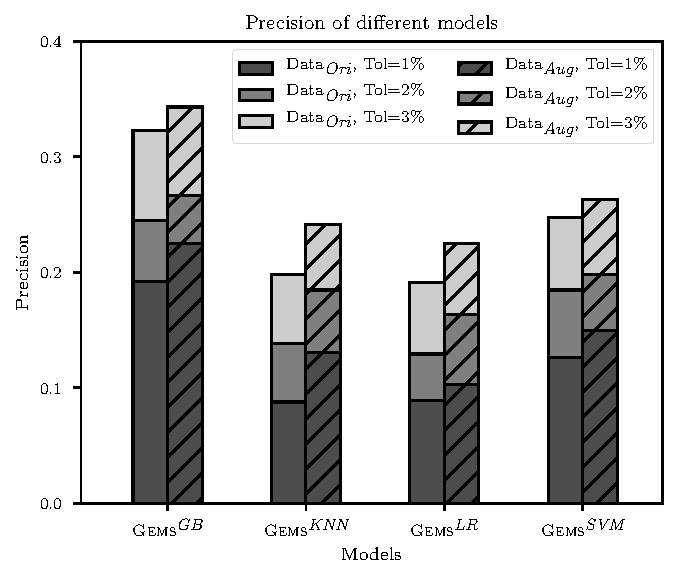
\includegraphics[width=0.49\linewidth]{Precision.pdf}}
\hfill
\subfigure[召回率]{\label{RQ3:recall}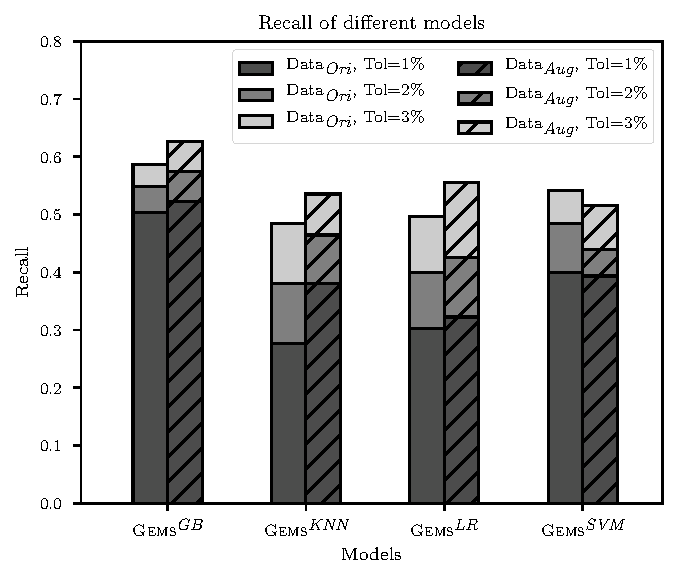
\includegraphics[width=0.49\linewidth]{Recall.pdf}}
\caption{训练数据集比较}
\label{dataset}
\end{figure}

图~\ref{dataset}为两组训练数据集在四个模型上的准确率和召回率。图~\ref{dataset}中斜条纹的柱形代表在扩
充数据集上的训练结果,没有斜条纹的柱形为在完全真实的数据上的训练结果;通过将容忍度设置为1\%、2\%和
3\%,得到在不同容忍度下模型的表现,在图~\ref{dataset}中依次用深灰色、灰色和浅灰色来表示。

通过观察图~\ref{dataset}中不同训练数据集的表现,可以得到以下结论:(1)在大部分情况下,使用扩充数据
集进行训练的模型表现优于使用原数据集训练得到的模型。只有在概率SVM模型中,原数据集的召回率略优于扩充
数据集,但该模型在扩充数据集上的准确率明显优于原数据集。这样的观察结果可能是因为扩充数据集的规模更
大,因此在大多数情况下具有更好的表现。(2)在KNN和LR中,扩充数据集对结果的改进要明显大于SVM和GBDT两个
模型。当使用原训练数据集时,LR和KNN的性能较差,可能是由于原数据集规模较小,由于数据不够多导致这两个
模型容易发生过拟合;而SVM由于最大间隔分类的原因,相比较LR和KNN不容易过拟合;类似的,GBDT为基于决策
树的融合模型,因此在小规模数据集上也能有较好的表现。

\subsection{梯度上升决策树和其它模型的比较}\label{RQ3}

\begin{figure}
\centering
\subfigure[准确率]{\label{RQ3:precision}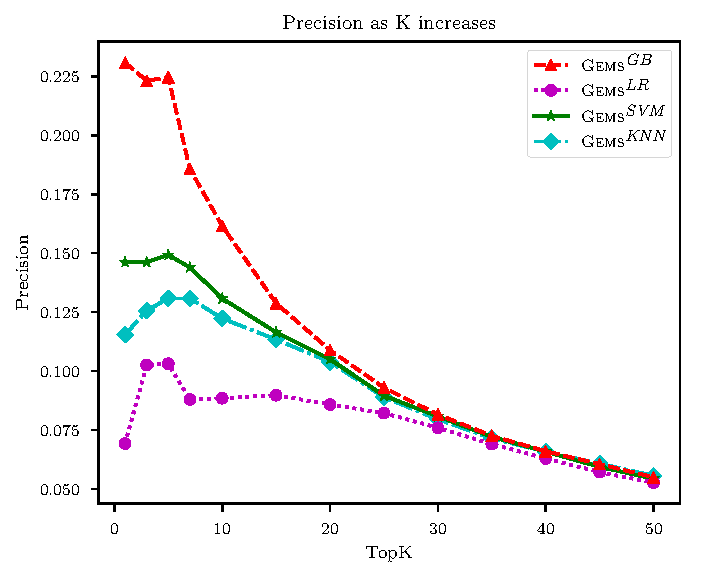
\includegraphics[width=0.49\linewidth]{topk_Precision.pdf}}
\hfill
\subfigure[召回率]{\label{RQ3:recall}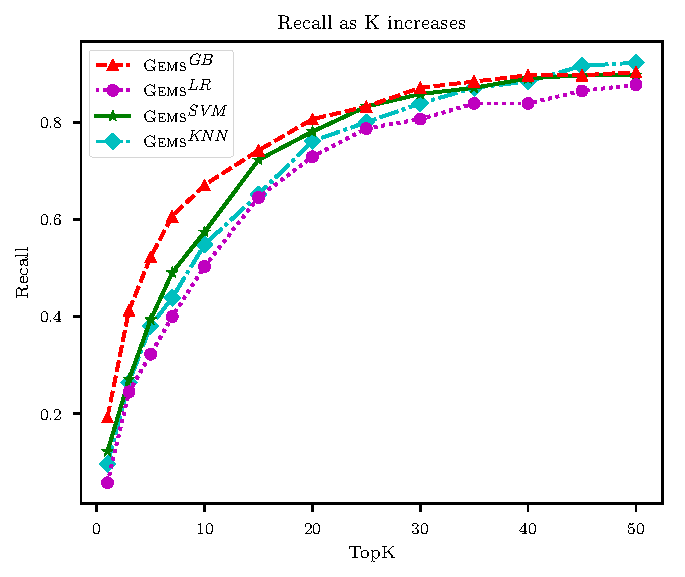
\includegraphics[width=0.49\linewidth]{topk_Recall.pdf}}
\caption{不同模型的准确率和召回率,横坐标表示推荐Top-$K$函数抽取重构机会}
\label{models1}
\end{figure}

为了评估梯度上升决策树模型在推荐函数抽取重构机会任务上的有效性,本节通过在不同特征组合上的表现来对以
下这四种模型进行对比。需要注意的是,虽然GEMS最终目的是为每个函数抽取重构机会预测其为正样本的概率,然
而两组训练数据集中都只包括正样本和负样本,因此对于部分无法直接预测类别概率的分类模型,还需要使用逻辑
斯特回归模型来做关于概率的训练,使分类器能够输出类别的概率。

具体来说,上述的四个模型中,只有梯度上升决策树和逻辑斯特回归模型可以直接预测给定样本为正例的概率,而最
近邻和支持向量机为分类模型,无法直接预测样本类别的概率。为了让分类器输出概率,在实验中使用逻辑斯特回
归,通过最大似然来拟合样本为正例的概率(Platt's scaling)。以概率SVM为例,传统的SVM针对给定测试样
本,根据训练好的参数计算出一个数值$y$,然后根据该数值是否大于0来预测该样本是否为正样本;概率SVM则以
第一阶段的输出$y$作为输入,样本的类别作为标签,通过逻辑斯特回归模型再训练,得到在输出为$y$时样本为正
例的概率。

图~\ref{models1}和图~\ref{models2}为当固定容忍度(1\%)和训练数据集(扩充数据集)时,GBDT、KNN、LR和
SVM四个模型的表现。其中红色代表GBDT,蓝色代表KNN,紫色代表LR,绿色代表SVM。横坐标为模型预测阶段,推
荐Top-$K$个函数抽取重构机会。从图~\ref{RQ3:recall}中可以看出,在大多数情况下GBDT的召回率略高于其它模
型;通过观察图~\ref{RQ3:precision}可以发现,GBDT的准确率相比较其它模型有很大优势,尤其推荐的函数抽取
重构机会较少时,GBDT的准确率明显高于其它模型。较高的准确率说明当推荐同样个数的函数抽取重构机会时,
GBDT模型推荐的模型更有可能被用户采纳,因此效率更高。

除此以外,通过观察图~\ref{models1}可以发现,当提高推荐的函数抽取重构机会数量时,召回率一直在上升,而
准确率则刚开始上升,达到峰值后迅速下降;最后当为每个函数推荐超过50个函数抽取重构机会时,召回率超过
92\%,而此时平均准确率降至0.05\%。图~\ref{models2}则更明显的反应了这一趋势,随着推荐的函数抽取重构机
会数量$K$的增加,F值先增长,大约当$K=5$时,四个模型的F值均达到峰值,然后随着$K$的增加,F值迅速降低。
基于以上观察,在实际使用GEMS的过程中,建议用户只看排名最高的5个函数抽取重构机会。

\begin{figure}
\centering
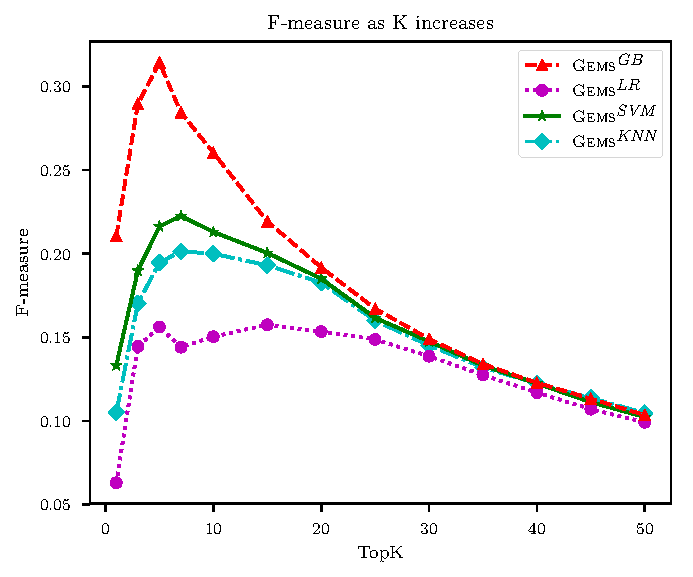
\includegraphics[width=0.49\linewidth]{topk_F-measure.pdf}
\caption{不同模型的F值,横坐标表示推荐Top-$K$函数抽取重构机会}
\label{models2}
\end{figure}

\subsection{针对长函数的实验结果}\label{RQ4}
由于函数抽取重构的目的之一是将长函数分解为短函数,因此本节针对实验数据集中的长函数进行对比实验。根据
之前的研究,长函数被定义为包括超过30行代码的函数~\cite{charalampidou2016identifying},表
~\ref{benchmark}中的实验对象一共包含15个长函数,涵盖了26个函数抽取重构机会。本节将GEMS与三种当前流行
的函数抽取重构推荐工具进行对比,评估GEMS处理长函数时的有效性。按照~\ref{canshu}中的参数设置方式,
GEMS、JExtract、SEMI和JDeodorant分别生成了1052、876、228和28个函数抽取重构机会。与之前的研究相同,为
每个函数最多保留排名最高的5个重构机会。表~\ref{long_methods}为在长函数上根据不同的容忍度统计得到的准
确率、召回率和F值。同样,黑体数值表示明显优于其它数值,而同等条件下的黑体数值之间相差在0.5\%以内,因
此被认为没有明显的区别。

通过观察表~\ref{long_methods}可以得到,在为长函数推荐函数抽取重构机会时,4个工具的结构均不如表
~\ref{accuracy}中的结果,说明了当面对长函数时,准确地推荐函数抽取重构机会存在一定的难度。不难发现,
当容忍度为1\%和2\%时,SEMI有最好的表现;当容忍度为2\%和3\%时,GEMS的表现最好。与表~\ref{accuracy}的
表现一样,JDeodorant由于其保守的函数抽取重构机会生成策略,准确率比JExtract高,同时JDeodorant的召回率
仍然是所有工具中最低的。当容忍度为1\%时,虽然GEMS的表现仍优于JExtract和JDeodorant,但其表现仍然不够
理想。然而,通过对实验数据进行分析,发现SEMI和GEMS对于长函数的表现差异,原因并不在于函数的规模,而在
于函数中存在的应该被抽取的函数片段较多。关于这个问题将在下一节中具体讨论。

\begin{table}[!t]
\zihaowu
  \renewcommand{\arraystretch}{1.3}
  % if using array.sty, it might be a good idea to tweak the value of
  % \extrarowheight as needed to properly center the text within the cells
  \caption{长函数准确性比较}
  \label{long_methods}
  \centering
  \begin{tabular}{cc|ccc}
  \toprule
   工具名称 &容忍度 &准确率 &召回率 &F值\\ 
  \midrule
  \multirow{4}{*}{GEMS$^{GB}$}&$1\%$ &13.3\% &31.9\% &18.8\% \\ 
  &$2\%$ &\bf{17.4\%} &\bf{41.5\%} &\bf{24.5\%} \\ 
  &$3\%$ &\bf{25.3\%} &\bf{46.2\%} &\bf{32.7\%} \\ 
  \hline
  \multirow{4}{*}{JExtract}&$1\%$ &6.6\% &16.1\% &9.4\% \\ 
  &$2\%$ &8.0\% &19.3\% &11.3\% \\ 
  &$3\%$ &8.0\% &19.3\% &11.3\% \\ 
  \hline
  \multirow{4}{*}{SEMI}&$1\%$ &\bf{16.4\%} &\bf{38.7\%} &\bf{23.0\%} \\ 
  &$2\%$ &\bf{17.9\%} &\bf{41.9\%} &\bf{25.0\%} \\ 
  &$3\%$ &19.1\% &45.1\% &26.9\% \\ 
  \hline
  \multirow{4}{*}{JDeodorant}&$1\%$ &12.0\% &9.6\% &10.7\% \\
  &$2\%$ &14.3\% &12.9\% &13.5\% \\ 
  &$3\%$ &16.0\% &12.9\% &14.2\% \\ 
  \bottomrule
  \end{tabular}
  \end{table}
  
\section{讨论}\label{discuss}
最后,本节就实验中发现的一些问题进行讨论。

\subsection{特征重要性}

尽管在实验中一共提取了48个特征进行训练,但这些特征的重要性并不完全相等。为了研究特征对实验结果的重要
性,使用过滤式特征选择(Relief特征选择算法)计算每个特征的相关统计量,然后使用不同的特征组合使用GBDT
进行训练。图~\ref{features}为使用不同数量的特征进行训练的实验结果,其中红色为召回率,绿色为准确率,
紫色表示F值。横坐标Top-$K$表示使用重要性最高的$K$个特征进行训练。

通过图~\ref{features}可以发现,当训练特征较少时,模型的表现较差。随着特征的数量逐渐增加,召回率、准
确率和F值随之增长。例如当特征的数量从5增加到35时,模型的准确率、召回率和F值分别提高了64.4\%、35.5\%
和55.8\%。然而,当继续增加特征的个数时,模型的表现逐渐降低。转折点大约出现在$K=35$处,因此有理由认为
并不是所有特征对模型训练都是有益的,48个特征中大约只有35个特征具有预测能力,而其它特征的加入只是引入
了噪音,可能导致模型效果降低。

  \begin{figure}
  \centering
  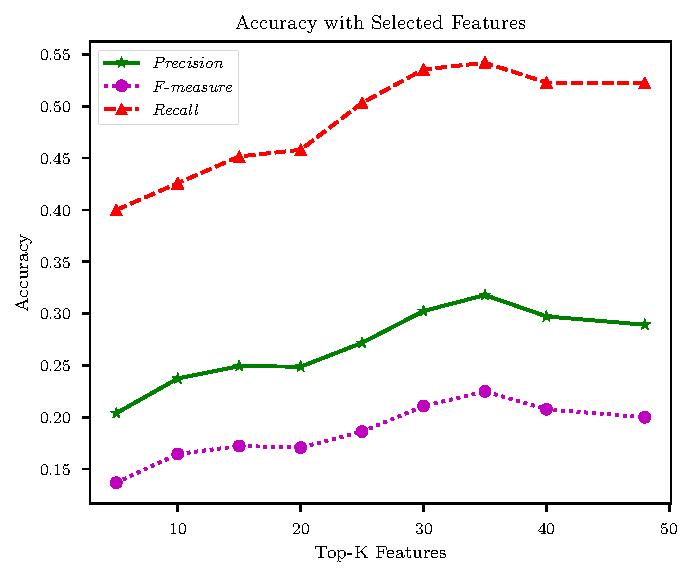
\includegraphics[width=0.49\linewidth]{fs.pdf}
    \caption{不同特征组合下的模型表现,横坐标表示使用Top-$K$个特征进行训练}
    \label{features}
  \end{figure}

表~\ref{important_features}中列出了按照特征重要性由高至低排名最高的20个特征。可以看到,排名较高的大
多为功能特征;特征``EXTRACTED\_LOCAL''的排名较高,意味着模型认为代码片段中是否含有本地变量的声明对决
定代码片段是否被抽取有较大影响;大多数与内聚度相关的特征(以``COHESION''结尾)在实验中被认为是比较重
要的。除此以外,表~\ref{important_features}中的排名说明了部分程序元素,如函数调用
(``INVOCATION'')、类型(``TYPE'')、包(``PACKAGE'')等比其它元素更重要,验证了本文研究动机中关于
软件质量度量由于考虑的程序元素较少,因此度量结果存在片面性的问题。

\begin{table}[!t]
\zihaowu
  \renewcommand{\arraystretch}{1.3}
  \caption{部分特征重要性排名}
  \label{important_features}
  \centering
  \begin{tabular}{p{1cm}c|p{1cm}c}
  \toprule 排名 &特征 &排名 &特征 \\ \midrule
  1& \textbf{INVOCATION\_COHESION}& 11& CON\_VAR\_ACC\\
  2& LOC\_EXTRACTED\_METHOD& 12& EXTRACTED\_LOCAL\\
  3& \textbf{TYPEDELE\_COHESION}& 13& CON\_LOC\\
  4& RATIO\_LOC& 14& EXTRACTED\_VAR\_AC\\
  5& CON\_PACKAGE& 15& \textbf{PACKAGE\_COHESION}\\
  6& EXTRACTED\_TYPED\_ELE& 16& CP\_PACKAGE\\
  7& CP\_VAR\_ACC& 17& CP\_PACKAGE2\\
  8& EXTRACTED\_PACKAGE& 18& \textbf{VARAC\_COHESION}\\
  9& \textbf{VARAC\_COHESION2}& 19& EXTRACTED\_IF\\
  10& CON\_INVOCATION& 20& EXTRACTED\_INVOCATION\\
  \bottomrule 
  \end{tabular}
  \end{table}
  
\subsection{多函数抽取重构机会}
通过观察针对长函数的实验数据,发现~\ref{RQ4}中所使用的长函数大多不止一个函数抽取操作(平均每个函数
1.9个),而GEMS的原理是预测候选函数抽取重构机会为正例的概率,并根据概率进行排序推荐。因此,不难理解,GEMS为相似的函数抽取重构机会分配相近的概率。同时,由于函数体内存在不止一个应该被抽取的代码片段,导致GEMS在为其中一个相关的函数抽取重构机会分配到高概率的同时,会为与其相似的其它重构机会分配较高的概率,因此导致其它不相似但应该被抽取的代码段的概率排名相对较低,最终导致了模型效率的下降。与GEMS相反,SEMI在推荐阶段将相似的函数抽取重构机会聚为一类,每次只从中选择排名最高的一个函数抽取重构机会进行推荐,从而取得了不错的表现结果。

针对上述问题,本文为使用者提供了两种策略:第一种,用户可以一步只进行一个函数抽取重构,在选定需要重构
的函数后,GEMS为用户推荐函数抽取重构机会列表,用户通过选择合适的重构机会让工具进行实施,在完成重构
后,若用户仍希望继续进行函数抽取,则再次选择该函数,进行下一轮的函数抽取重构推荐,直到使用者放弃重构
为止;(2)基于与SEMI类似的思路,可以将相似的函数抽取重构机会放到一组中,对于每组只推荐概率最高的函
数抽取重构机会给用户。具体来说,如果两个函数抽取重构机会$a$和$b$满足以下条件,则认为它们较为相似,可
以被放到一组:
\begin{eqnarray}
  \frac{\lvert{Start_a - Start_b}\rvert + \lvert{End_a - End_b}\rvert}{MAX(LoC_a, LoC_b)}\leq \it Threshold,
\end{eqnarray}
其中$Start$和$End$分别表示待抽取代码的起止行号;LOC为待抽取代码的行数,$Threshold$为设定的阈值。

\section{本章小结}
本章提出了基于梯度上升决策树的函数抽取重构机会推荐方法,并基于该方法开发了Eclipse插件GEMS。在训练阶
段,该方法首先每个训练样本提取两组特征,分别是结构特征和功能特征,融合了复杂度、内聚度和耦合度三个重
要的软件质量因素,以及多种与函数抽取重构相关的程序元素,并利用梯度上升决策树模型训练。在推荐阶段,针
对给定函数,首先使用基于代码块的方法生成所有合法的函数抽取重构机会,然后使用训练好的模型为每个函数抽
取重构机会分配一个概率,并根据概率由高至低推荐给用户。

通过在开源软件上进行实验,发现尽管GEMS生成了大量的函数抽取重构机会,但使用训练好的模型可以为好的函数
抽取重构机会分配较高的概率,使其排名较高,从而在实验中具有较好的表现。除此以外,受变异测试启发,本
文提出了使用函数内联重构来扩充训练数据集,并通过实验证明该训练集在大多数情况下能够取得比原训练数据集
更好的结果。值得注意的是,本文在构造扩充数据集时,谨慎地选择了具有良好设计模式的开源程序,并且只内联
被调用一次的函数作为待抽取片段,认为通过将该代码片段重新抽取出来能够提高程序的易读性、可维护性和可靠
性,与函数抽取的主要目的相一致。最后在不同模型上的实验结果证明了梯度上升决策树在推荐函数抽取重构机会
时的有效性,尤其当使用原数据集时,由于其融合模型的性质使得在小规模数据集上,该模型相比较其它三种模型
有较为明显的优势。通过分析特征重要性,本文发现了对函数抽取重构较为重要的因素,对了解函数抽取重构的意
图有一定程度的帮助。

本章具有以下贡献:

(1)提出了一个关于函数抽取重构的概率模型,通过学习从开源软件仓库中挖掘到的重构实例,模拟了软件维护
人员进行软件重构的过程,并考虑了函数抽取重构原因的多样性。

(2)提出了关于结构特征和功能特征的特征提取算法,融合了内聚度、耦合度、复杂度的软件质量概念,并考虑
了多种程序元素。

(2)设计并开发了一个基于Eclipse的插件GEMS,为给定Java函数生成函数抽取重构机会,并为每个合法的候选重
构机会分配一个概率,按照概率由高至低推荐给集成开发环境使用者。

(3)在开源程序上与主流函数抽取重构推荐工具的对比实验证明了GEMS的有效性,能够更准确地推荐函数抽取重
构机会,为软件维护人员提高维护效率。